\scanpage{43}
[\uline{Ex} $n=1$, $\rho=4-\beta=2-\alpha$, $\sigma=\deleted{\unsure{alors}}2$,
$\widetilde\sigma=1$. Donc

\deleted{\unsure{Par}} $1^\circ)$ si $\deleted{\unsure{2}}\rho$ inv.
\inserted{i.e. $U_\rho\simeq\mathbb G_m$},
\deleted{alors} $\exists!$ $u\in U_{\rho=2-\alpha}$ partout $\ne1$,
telle que $u$ invarie $f^{\mathcal E}$ (--- ce qui revient au $=$,
\deleted{$\unsure{Q_X}$} la conique $Q_X$)
savoir l'antipodisme, qui est l'unique section $u$ telle que
$u^2=1$, $u_s\ne1$ $\forall s\in S$.

$2^\circ)$ Conditions équivalentes

a) $\rho=0$ et \deleted{\unsure{sur}} $S$ de car $2$ $(2.1_S=0)$

b) $U_\rho$ invarie $f^{\mathcal E}$

c) $U_\rho$ --- $Q_X$

d) $\rho=0$ et $\exists$ loc. section partout $\ne1$,
qui invarie $f^{\mathcal E}$ (ou encore, $Q_X$). ]

\figure{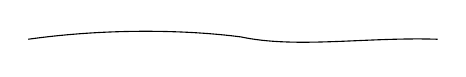
\begin{tikzpicture}
\draw (0,0)..controls(1,.14)and(2,.12)..(2.7,.03)..controls(3.4,-.12)and(4.3,.03)..(5.2,0);
\end{tikzpicture}}

\uline{Proposition}\quad 1) Si $\sigma\widetilde\rho$ inversible,
$\exists!$ section $u$ de $U_\rho$, partout $\ne1$, qui invarie $f^{\mathcal E}$
i.e. $Q_X$, savoir l'antipodisme.

2) Conditions équivalentes

a) $\sigma=0$ et $\widetilde\sigma\widetilde\rho=0$
\margin{(cette dernière condition conséquence de la première si $n$ pair ou $2$ inv.)}

b) $U_\rho$ invarie $f^{\deleted{\unsure{\mathcal E}}\inserted{\mathcal E}}$

c) $U_\rho$ invarie $Q_X$

\margin{\unsure{?}}
d) (\uuline{Si $\widetilde\sigma\widetilde\rho=0$})
$\exists$ loc. section de $U_\rho$ partout $\ne1$, qui invarie $f^{\mathcal E}$
(ou $Q_X$)
\mspage{42}

